\documentclass[preview]{standalone} 
\usepackage[tikz,plot,math]{forsyde}
\usepackage{amsmath}
\usepackage{array}
\usepackage[layered]{forsyde-pictures}
\usepackage{forsyde-atom-docs}

\begin{document}


\begin{docimage}{process-constructor}
  \begin{tabular}[t]{m{6cm}m{9cm}}
  \vbox{\begin{align*}
    p_1(s_1) &= (+) \MocFun s_1 \\
    p_2(s_1,s_2) &= s_1 \MocApp s_2 \\
    pn(s_1,s_2) &= (p_2(s_2) \circ p_1)(s_1) \\    
    pc'(f)(s_1, s_2) &= (\MocApp\, s_2) \circ (f \MocFun s_1) \\
    p'(s_1,s_2) &= pc'\, (+) (s_1,s_2) \\
    pn &\equiv p'
  \end{align*}}
  &
    \begin{tikzpicture}[]
      \basic[primitive,
      f=$(\alpha\rightarrow\beta\rightarrow\gamma)$](p1)<0,1>{$\MocFun$};
      \basic[primitive](p2)<1,0>{$\MocApp$};
      \node[anchor=south east] (in1) at ($(p1)-(1,0)$) {$\mathcal{S}(\alpha)$};
      \node[anchor=south east] (in2) at ($(p2)-(2,0)$) {$\mathcal{S}(\beta)$};
      \node[anchor=south west] (out) at ($(p2)+(1,0)$) {$\mathcal{S}(\gamma)$};
      \node[anchor=west] (inter) at ($(p1)!.2!(p2)$) {$\mathcal{S}(\beta\rightarrow\gamma)$};
      \signal[] (in1.south west) -> (p1);
      \signal[] (in2.south west) -> (p2);
      \signal[] (p1) -> (p2);
      \signal[] (p2) -> (out.south east);
    \end{tikzpicture}
  \end{tabular}
\end{docimage}


\begin{docimage}{tagged-signal}
  \begin{equation*}
    \begin{split}
      &s = \{e_0, e_1,...\} \in S\\
      &\begin{split}
        \text{where } & e_j = (t_j, v_j)\\
        & v_j \in V,\ t_j \in T \\
        & t_j \leq t_{j+1},\ \forall\ j \in \mathbb{N}
      \end{split}
    \end{split}
  \end{equation*}
\end{docimage}


\begin{docimage}{ct-model}
  \begin{tikzpicture}[con/.style={circle,fill=black,inner sep=1pt}]
    \draw[ultra thick] (0,.5) node[con] (i1) {} -- (1,0) node[con] (o1) {};
    \draw[-latex] (.6,.5) node[anchor=south west] {\scriptsize$t=3$} to[bend right] (.3,-.2);
    \node[con] (i2) at (0,-.5) {};
    \begin{signalsCT}[timestamps=2, grid=2, xshift=-1cm,
      anchor=east, signal sep=1.5]{6}
      \signalCT*[outline,ordinate=0,ymin=-1,ymax=1]{%
        data/ct-subsig-s1.flx}
      \signalCT*[outline,ordinate=0,ymin=-1,ymax=1]{%
        data/ct-subsig-s2.flx}
    \end{signalsCT}
    \signal[] (sigplot.e1) -> (i1);
    \signal[] (sigplot.e2) -> (i2);
    
    \begin{signalsCT}[timestamps=2, grid=2, xshift=1cm,
      anchor=west, at={o1}]{6}
      \signalCT*[outline,ordinate=0,ymin=-1,ymax=1]{%
        data/ct-subsig-s3.flx}
    \end{signalsCT}
    \signal[] (o1) -> (sigplot.w1);  
  \end{tikzpicture}
\end{docimage}

\begin{docimage}{layered-model}
\begin{tikzpicture}
  \forsydeAtomMakeLayers[]{%
    Function Layer:Function,%
    Behavior Layer:Behavior,%
    MoC Layer:Process,%
    Skeleton Layer:Process Network}
  \node[] (value) at (layer0-center){%
    \usebox{\forsydeAtomValue}};
  \node[] (ext-value) at ($(layer1-center)!.5!(layer2-center)$) {%
    \usebox{\forsydeAtomExtValue}};
  \node[] (event) at ($(layer2-center)!.5!(layer3-center)$) {%
    \usebox{\forsydeAtomTagExtValue}};
  \forsydeAtomSignalArrow[width=4.2cm]{layer3-center}
  \node[inner sep=0] (token) at (arrow-center) {%
    \usebox{\forsydeAtomTagExtValue}};
  \node[] at ($(token.east)!.5!(arrow-west)$) {%
    \usebox{\forsydeAtomTagExtValue}};
  \node[] at ($(token.west)!.5!(arrow-east)$) {%
    \usebox{\forsydeAtomTagExtValue}};
  \forsydeAtomSignalVector{layer4-rightpath}
  \node[anchor=north] at (arrow-south) {\emph{Regular structure of signals}};
  \node[anchor=north] at (event.south west) {\footnotesize Tagged event};
  \node[anchor=north] at (ext-value.south west) {\footnotesize Extended value};
  \node[anchor=north] at (value.south west) {\footnotesize Value};

  \node[anchor=north , text width=5em, yshift=-15pt, xshift=-75pt, font=\scriptsize] at (event.west) {Describes: \\ 
    $\bullet$ recursive patterns of processes \\ 
    $\bullet$ inherently parallel networks};
  \node[anchor=north , text width=4.7em, yshift=-30pt, xshift=-25pt, font=\scriptsize] at (event.south west) {Describes: \\ 
    $\bullet$ MoC semantics \\ 
    $\bullet$ time behavior \\ 
    $\bullet$ synchronization};
  \node[anchor=north , text width=4.8em, yshift=-14pt, xshift=-18pt, font=\scriptsize] at (ext-value.south west) {Describes: \\ 
    $\bullet$ extended value semantics \\ 
    $\bullet$ behavior in case of special events};
  \node[anchor=east, text width=5em, font=\scriptsize] at (value.west) {Exposes functionality};
\end{tikzpicture}
\end{docimage}


\begin{docimage}{process}
  \begin{equation*}
    \begin{array}{l}
      p : S^m \rightarrow S^n \in P\\
      p (s,...)= (s,...)
    \end{array} 
    \qquad    
    \begin{array}{l}
      pc_{\text{M}} : V^n \rightarrow P \in PC\\
      pc_{\text{M}} (v,...)= p
    \end{array} 
  \end{equation*}
\end{docimage}

\begin{docimage}{ser-composition}
  \begin{tabular}[t]{m{6cm}m{9cm}}
    \vbox{
    \begin{align*}
      p_1 &: S_\alpha \rightarrow S_\beta \\
      p_2 &: S_\beta \rightarrow S_\gamma \\
      p_2 \circ p_1 &: S_\alpha \rightarrow S_\gamma \\
      (p_2 \circ p_1)&(s)\equiv p_2(p_1(s))
    \end{align*}}
  &
    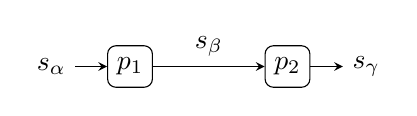
\begin{tikzpicture}[baseline={(sa.south)}, every node/.style={rounded corners=3pt}]
      \node[draw, minimum size=15pt] (p1) at (0,0) {$p_1$}; 
      \node[draw, minimum size=15pt] (p2) at (2,0) {$p_2$};
      \node[] (sa) at (-1,0) {$s_\alpha$}; 
      \node[anchor=south] (sb) at (1,0) {$s_\beta$}; 
      \node[] (sg) at (3,0) {$s_\gamma$};
      \draw[-stealth] (sa) -- (p1); \draw[-stealth] (p1) -- (p2);
      \draw[-stealth] (p2) -- (sg);
    \end{tikzpicture}
  \end{tabular}
\end{docimage}

\begin{docimage}{unzip}
\begin{tabular}[t]{m{7cm}m{9cm}}
  \vbox{\begin{align}
    \id{pc} &: (\alpha\rightarrow\beta^n) \rightarrow \mathcal{S}(\alpha) \rightarrow \mathcal{S}(\beta^n)  \\
    \triangleleft &: \mathcal{S}(\beta^n) \rightarrow \mathcal{S}(\beta)^n \\
    (pc\,f \triangleleft) &:  \mathcal{S}(\alpha) \rightarrow \mathcal{S}(\beta)^n
  \end{align}}
  &
  \begin{tikzpicture}[]
    \basic[primitive](p3)<3,0>{$\triangleleft$};
    \node[] (in3) at ($(p3)-(1.5,0)$) {$\mathcal{S}(\beta^n)$};
    \node[] (ou1) at ($(p3)+(2,2.25)$) {$\mathcal{S}(\beta_1)$};
    \node[] (ou2) at ($(p3)+(2,1.5)$) {$\mathcal{S}(\beta_2)$};
    \node[] (ou3) at ($(p3)+(2,0)$) {$\mathcal{S}(\beta_n)$};
    \node[] at ($(ou2)!.5!(ou3)$) {$\vdots$};
    \signal[] (in3) -> (p3);
    \signal[] (p3) - (4,2.25); \signal[] (4,2.25) -> (ou1);
    \signal[] (p3) - (4,1.5); \signal[] (4,1.5) -> (ou2);
    \signal[] (p3) -> (ou3);
  \end{tikzpicture}
\end{tabular}
\end{docimage}

\end{document}

%%% Local Variables:
%%% TeX-command-default: "Make"
%%% mode: latex
%%% TeX-master: t
%%% End:
